\documentclass{article}
\usepackage[a4paper, margin={25mm,30mm}]{geometry}
\usepackage[italian]{babel}
\usepackage{hyperref}
\usepackage{graphicx}
\usepackage{minted}
\usepackage{dirtree}

\author{Diego Roberto Ammirabile 0001021216 \\ \texttt{diego.ammirabile@studio.unibo.it}}
\date{Febbraio 2025}
\title{Report}
\begin{document}
\maketitle
\tableofcontents

\section{Panoramica del progetto}
\subsection{Obiettivi}
Il progetto ha implementato le seguente funzionalità:
\begin{itemize}
    \item registrazione e login dell'utente
    \item salvataggio e gestione della scadenza del token di autenticazione
    \item registrazione di audio
    \item memorizzazione di audio registrati su database locale SQLite
    \item visualizzazione di audio registrati
    \item caricamento di audio registrati sull'API
    \item eliminazione di audio registrati dal database locale e dall'API
    \item geolocalizzazione dell'utente
    \item visualizzazione di audio sulla mappa con relative informazioni
    \item visualizzazione di informazioni dell'audio salvato
    \item caricamento posticipato degli audio
    \item implementazione mostra/nascondi audio sulla mappa
\end{itemize}
Da specifiche erano richieste ulteriori funzionalità, tuttavia non sono state implementate a causa di problemi tecnici e di tempo. Questo argomento verrà trattato più avanti nelle conclusioni.
\section{Dettagli di implementazione}
Il progetto è stato realizzato attraverso grazie al framework \texttt{Ionic} combinato con il framework \texttt{Vue}, quindi l'applicazione è stata sviluppata utilizzando MVVM come design pattern. Quando possibile è stato utilizzato il \texttt{Capacitor} per accedere alle funzionalità native dei dispositivi mobili, questo non è sempre stato possibile a causa di limitazioni del framework. Per avere una migliore gestione dei tipi è stato utilizzato \texttt{TypeScript}. Il progetto è stato inizializzato con \texttt{Vite}.

Ionic è stato scelto poiché permette di ``riciclare" le conoscenze di programmazione web e la familiarità con i framework javascript, inoltre permette di generare applicazioni per più piattaforme con un unico codice sorgente, caratteristica che però non è stata sfruttata.

Una comodità da non sottovalutare è la leggerezza dell'ambiente di sviluppo comparata ad \textit{Android Studio} o \textit{XCode}, inoltre la possibilità di utilizzare un browser per testare l'applicazione è un vantaggio non da poco.

Esistono in oltre delle librerie di componenti già pronti, che permettono di velocizzare lo sviluppo e si possono sfruttare le librerie sviluppate per javascript/typescript. Tuttavia non sempre funzionano correttamente e spesso è necessario apportare modifiche.

\subsection{Struttura del codice}
Il codice è stato organizzato in componenti Vue, in modo da rendere il codice più modulare e manutenibile. Ogni componente è stato progettato per essere il più possibile indipendente dagli altri, in modo da poter essere riutilizzato in altri contesti. Esistono tuttavia componenti che non trovano applicazione in altri contesti se non quello del sovra-componente, tali componenti però gestiscono parti di logica differente da quella del sovra-componente, per cui è stato ritenuto utile mantenerli separati.
Il filesystem ha quindi la seguente struttura:
\begin{itemize}
    \item \texttt{android/} contiene i file necessari per la compilazione dell'applicazione per Android
    \item \texttt{dist/} contiene i file compilati
    \item \texttt{node\_modules/} contiene le dipendenze del progetto
    \item \texttt{public/} contiene i file statici
    \item \texttt{src/} contiene il codice sorgente
        \begin{itemize}
            \item \texttt{components/} contiene i componenti Vue
            \item \texttt{router/} contiene il router
            \item \texttt{theme/} contiene i file di stile
            \item \texttt{utils/} contiene le utility
            \item \texttt{views/} contiene le viste
            \item \texttt{App.vue} è il file principale
            \item \texttt{interfaces.ts} contiene le interfacce
            \item \texttt{main.ts} è il file principale
            \item \texttt{variables.json} contiene le variabili, di fatto solo l'URL dell'API
            \item \texttt{vite-env.d.ts} contiene le variabili di ambiente
        \end{itemize}
    \item \texttt{capacitor.config.ts} contiene la configurazione di Capacitor
    \item \texttt{cypress.config.ts} contiene la configurazione di Cypress
    \item \texttt{index.html} è il file principale
    \item \texttt{ionic.config.json} contiene la configurazione di Ionic
    \item \texttt{LICENSE} contiene la licenza
    \item \texttt{package-lock.json} contiene le dipendenze con le versioni esatte
    \item \texttt{package.json} contiene le dipendenze
    \item \texttt{ProjectsLAM2024.pdf} contiene il progettato
    \item \texttt{README.md} contiene le informazioni sul progettato
    \item \texttt{tsconfig.json} contiene la configurazione di TypeScript
    \item \texttt{tsconfig.node.json} contiene la configurazione di TypeScript per Node
    \item \texttt{vite.config.ts} contiene la configurazione di Vite
\end{itemize}

\subsection{Viste}
Nella cartella \texttt{src/views/} sono presenti le viste dell'applicazione, queste sono state progettate per gestire una parte della logica dell'applicazione, in modo da rendere il codice più manutenibile e modulare.
Le viste vengono caricate tramite il router che si trova nel file \texttt{src/router/index.ts}. A seconda delle viste è stata scelto se caricare i componenti in modo sincrono o asincrono, in modo da velocizzare il caricamento dell'applicazione. Per esempio la vista di login è caricata in modo sincrono nel seguente modo:
\begin{minted}{typescript}
{
    path: '/login',
    name: 'login',
    component: LoginPage
}
\end{minted}
mentre la vista della mappa, più impegnativa dal punto di vista delle risorse, è caricata in modo asincrono nel seguente modo:
\begin{minted}{typescript}
{
    path: 'tab2',
    component: () => import('@/views/MapPage.vue')
},
\end{minted}

\subsection{Componenti}
Nella cartella \texttt{src/components/} sono presenti i componenti dell'applicazione, questi sono stati progettati per evitare ripetizione di codice e per rispecchiare un'unità logica dell'applicazione.
La struttura dei componenti è la classica struttura di un componente Vue:
\begin{minted}{Vue}
<template>
<!-- HTML -->
</template>
<script setup lang="ts">
// TypeScript
</script>
<style scoped>
/* CSS */
</style>
\end{minted}

\subsubsection{Componente Audio e sotto-componenti}
Il componente \texttt{Audio} è il componente più complesso dell'applicazione, è stato progettato per gestire la registrazione e la visualizzazione degli audio. Questo componente è composto da diversi sotto-componenti, che gestiscono parti della logica differenti. La sua view ha la seguente struttura:
\begin{minted}{Vue}
<template>
  <div id="card" v-if="visible">
    <div id="base-info">
      <IonButton fill="clear" @click="playFunction">
        <IonIcon :icon="playIcon" :disabled="props.audio.audioBase64==''"></IonIcon>
      </IonButton>
      <AudioTimestamp :duration="props.audio.duration" ref="timestamp"/>
      <AudioPreview :audio="audio" v-if="!props.audio.metadata" @delete="deleted" 
      @upload="(uploadedAudio) => {props.audio.metadata = uploadedAudio.metadata}"/>
      <AudioUploaded :audio="audio" v-else @delete="deleted" @showMoreInfo=
      "toggleMoreInfo" />
    </div>
    <MetadataInfo :metadata="metadata" v-if="moreInfoVisible && metadata"/>
  </div>
</template>
\end{minted}

tra i sotto-componenti vanno annoverati \texttt{AudioTimestamp} che si occupa di mostrare lo scorrere del tempo durante l'ascolto (è anche utilizzato per visualizzare lo correre del tempo durante la registrazione), \texttt{AudioPreview} che visualizza la parte dell'interfaccia visualizzata per gli audio non caricati e \texttt{AudioUploaded} che visualizza la parte dell'interfaccia visualizzata per gli audio caricati.

\texttt{MetadataInfo} è un componente che visualizza le informazioni dell'audio, è utilizzato sia per visualizzare le informazioni degli audio registrati dall'utente, sia per visualizzare le informazioni degli audio registrati dagli altri utenti. Nel componente è presente un bottone per mostrare/nascondere le informazioni dell'audio.



\subsection{utility}
Nella cartella \texttt{src/utils/} sono presenti le utility dell'applicazione, queste sono state progettate per evitare ripetizione di codice e per rispecchiare un'unità logica dell'applicazione, in una certa misura ogni file corrisponde a un model, quando questo è utile a più componenti. Questi sono in paricolare i file:

% audio_processing.ts
% geolocation.ts
% hash.ts
% requests.ts
% storage.ts

\begin{itemize}
    \item \texttt{audio\_processing.ts} contiene le funzioni per la conversione dei codec audio tramite \texttt{FFmpeg} implementato in \texttt{WebAssembly} \footnote{FFmpeg è implementato in WebAssembly da \url{https://www.npmjs.com/package/@ffmpeg/ffmpeg}}
    \item \texttt{geolocation.ts} contiene le funzioni per la geolocalizzazione, implementate tramite Capacitor \footnote{La geolocalizzazione è implementata tramite la libreria di Capacitor \url{https://capacitorjs.com/docs/apis/geolocation}}
    \item \texttt{hash.ts} contiene le funzioni per l'hashing delle password, implementate tramite \texttt{typescript}
    \item \texttt{requests.ts} contiene le funzioni per le richieste all'API, implementate tramite \texttt{Capacitor}
    \item \texttt{storage.ts} contiene le funzioni per la gestione del database locale, implementate tramite \texttt{Capacitor} \footnote{Il database locale è implementato tramite la libreria della comunità di Capacitor \url{https://npmjs.com/package/@capacitor-community/sqlite}}
\end{itemize}

\section{Interfaccia utente}

% login.png
% signup.png
% record.png
% recorded-audio.png
% redorded-uploaded.png
% map-pins.png
% map-audio-info.png
% map-audio-submenu.png
% saved.png
% saved-infos.png

\subsection{Login e registrazione}
La prima schermata che si presenta all'utente è quella di login, questa pagina contiene anche il collegamento alla pagina di registrazione dell'utente. È possibile salvare le credenziali dell'utente per evitare di doverle inserire ogni volta.\footnote{ Le credenziali sono salvate tramite \url{https://capacitorjs.com/docs/apis/preferences}} Questa schermata è mostrata in figura \ref{fig:login}. La schermata di registrazione è mostrata in figura \ref{fig:signup}.
\begin{figure}[H]
    \begin{minipage}{0.48\textwidth}
        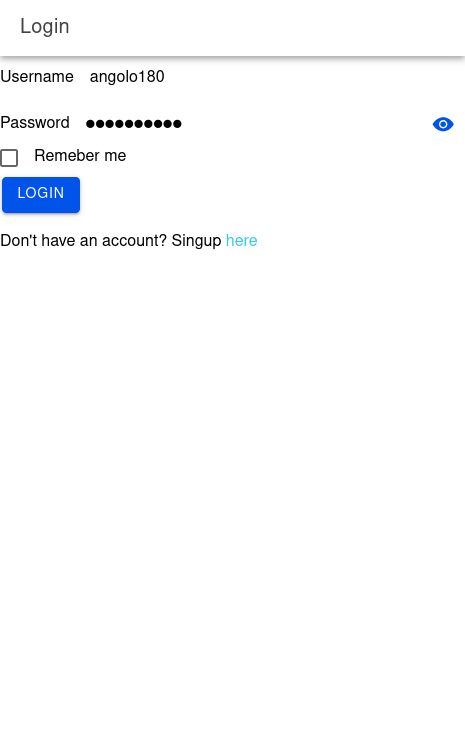
\includegraphics[width=\linewidth]{login.png}
        \centering
        \caption{Schermata di login}
        \label{fig:login}
    \end{minipage} \hfill
    \begin{minipage}{0.48\textwidth}
        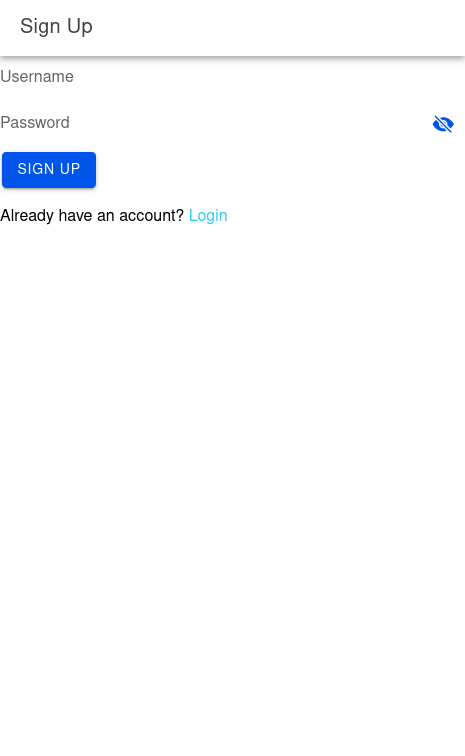
\includegraphics[width=\linewidth]{signup.png}
        \centering
        \caption{Schermata di registrazione}
        \label{fig:signup}
    \end{minipage}
\end{figure}

\subsection{Registrazione audio}
La schermata di registrazione audio è mostrata in figura \ref{fig:record}. Questa schermata permette di registrare audio e di salvarlo nel database locale. È possibile ascoltare l'audio registrato prima di caricarlo sull'API. La schermata di registrazione audio con audio registrato è mostrata in figura \ref{fig:recorded-audio}, mentre la schermata di registrazione dopo che l'audio è stato caricato sull'API è mostrata in figura \ref{fig:redorded-uploaded}.

\begin{figure}[H]
    \begin{minipage}{0.30\textwidth}
        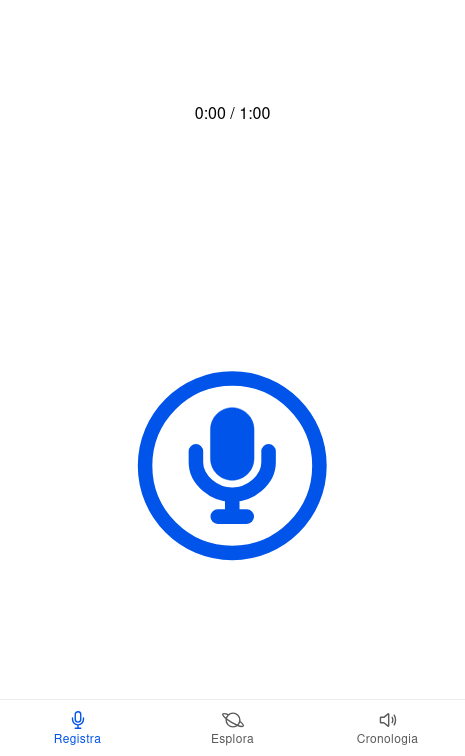
\includegraphics[width=\linewidth]{record.png}
        \centering
        \caption{Schermata di registrazione audio}
        \label{fig:record}
    \end{minipage} \hfill
    \begin{minipage}{0.30\textwidth}
        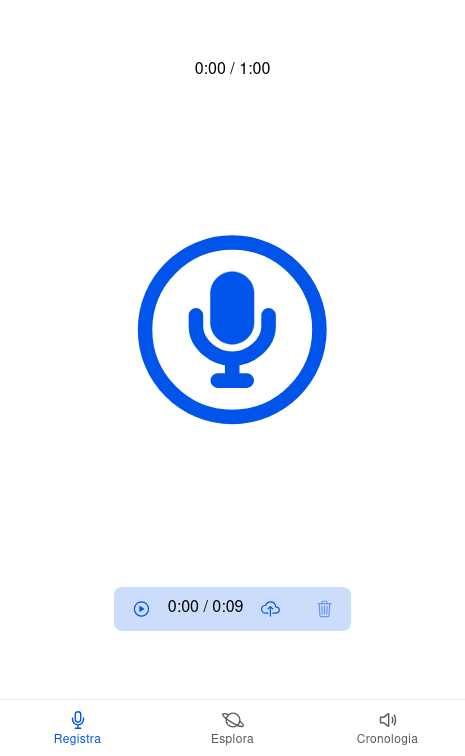
\includegraphics[width=\linewidth]{recorded-audio.png}
        \centering
        \caption{Schermata di registrazione audio con audio registrato}
        \label{fig:recorded-audio}
    \end{minipage} \hfill
    \begin{minipage}{0.30\textwidth}
        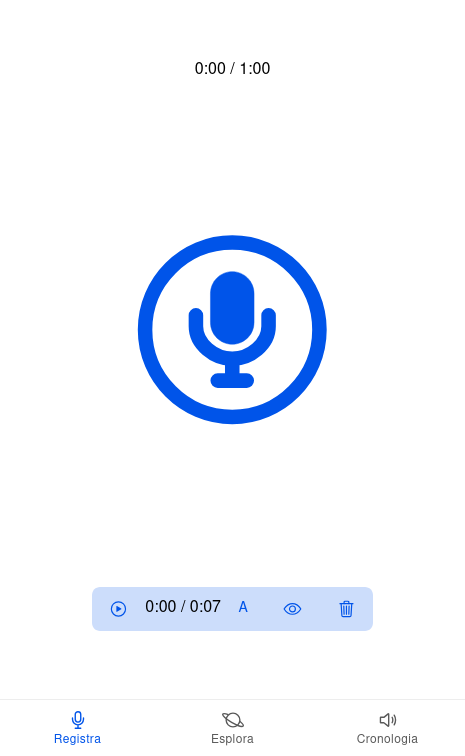
\includegraphics[width=\linewidth]{redorded-uploaded.png}
        \centering
        \caption{Schermata di registrazione audio con audio caricato}
        \label{fig:redorded-uploaded}
    \end{minipage}
\end{figure}

\subsection{Mappa}
La schermata della mappa con i pin è mostrata in figura \ref{fig:map-pins}. Questa schermata permette di visualizzare gli audio registrati sulla mappa. La mappa è stata realizzata tramite \texttt{Leaflet} \footnote{Leaflet è una libreria per la creazione di mappe interattive \url{https://leafletjs.com/}}, non si trattato di un componente nativo, ma ciononostante è stato preferito a \texttt{Google Maps}, che dispone di una implementazione nativa \footnote{Google Maps dispone di una implementazione nativa ufficiale di Capacitor; link alla documentazione: \url{https://capacitorjs.com/docs/apis/google-maps}} l'interfaccia è più pulita, la documentazione è più chiara ed è più facilmente personalizzabile.

È possibile visualizzare le informazioni degli audio registrati cliccando sul pin, come mostrato in figura \ref{fig:map-audio-info}. Le informazioni mostrate sono ricavate dall'API e il componente utilizzato per visualizzare le informazioni lo stesso usato per la visualizzazione delle informazioni degli audio del utente caricato, mostrata in figura \ref{fig:saved-infos}.

È possibile visualizzare più informazioni sul file audio cliccando sui menù a tendina dell'audio registrato, come mostrato in figura \ref{fig:map-audio-submenu}.

\begin{figure}[H]
    \begin{minipage}{0.30\textwidth}
        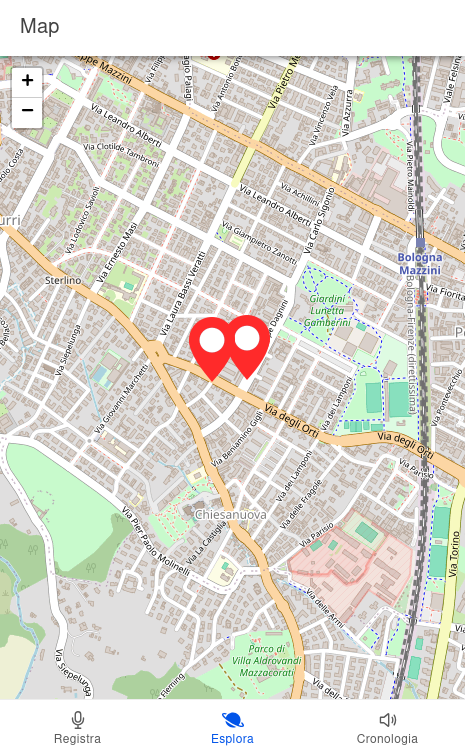
\includegraphics[width=\linewidth]{map-pins.png}
        \centering
        \caption{Schermata della mappa con i pin}
        \label{fig:map-pins}
    \end{minipage} \hfill
    \begin{minipage}{0.30\textwidth}
        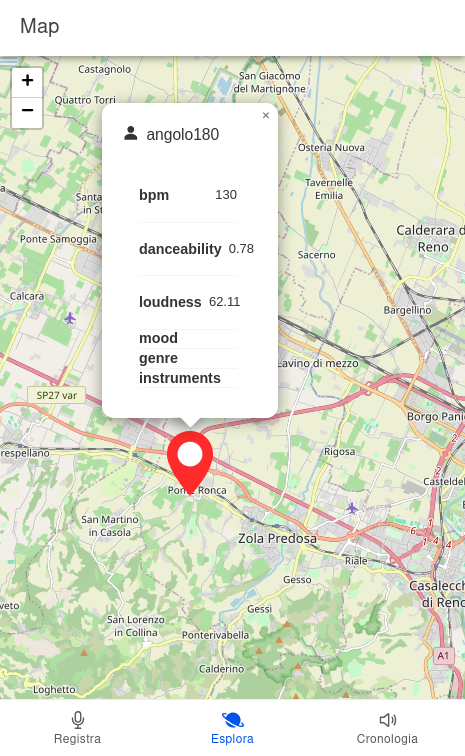
\includegraphics[width=\linewidth]{map-audio-info.png}
        \centering
        \caption{Schermata della mappa con le informazioni dell'audio}
        \label{fig:map-audio-info}
    \end{minipage} \hfill
    \begin{minipage}{0.30\textwidth}
        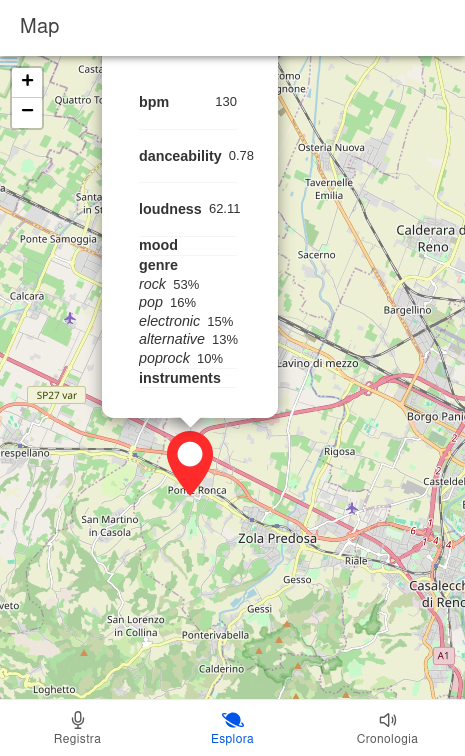
\includegraphics[width=\linewidth]{map-audio-submenu.png}
        \centering
        \caption{Schermata della mappa con un sotto-menu aperto}
        \label{fig:map-audio-submenu}
    \end{minipage}
\end{figure}

\subsection{Audio salvati}
La schermata degli audio salvati è mostrata in figura \ref{fig:saved}. Questa schermata permette di visualizzare gli audio registrati dall'utente. È possibile visualizzare le informazioni degli audio registrati cliccando sulla lettera ``A", come mostrato in figura \ref{fig:saved-infos}. Inoltre gli audio salvati sono riascoltabili, cancellabili e, qualora non siano stati caricati sull'API, è possibile caricarli.

Infine è possibile nascondere gli audio agli altri utenti, tramite l'icona dell'occhio.

\begin{figure}[H]
    \begin{minipage}{0.48\textwidth}
        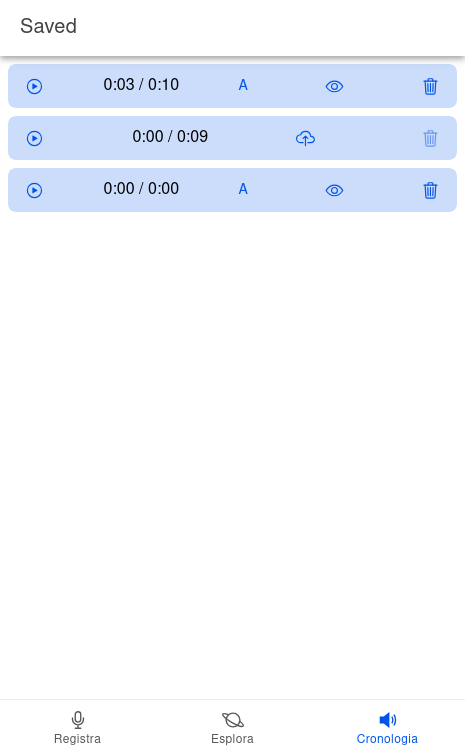
\includegraphics[width=\linewidth]{saved.png}
        \centering
        \caption{Schermata degli audio salvati}
        \label{fig:saved}
    \end{minipage} \hfill
    \begin{minipage}{0.48\textwidth}
        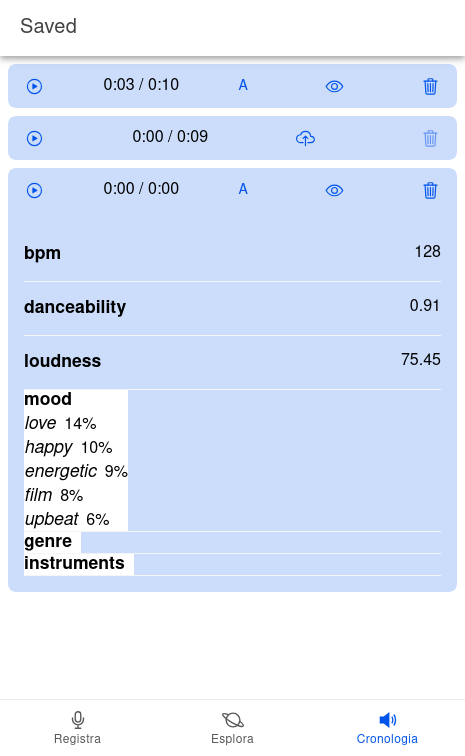
\includegraphics[width=\linewidth]{saved-infos.png}
        \centering
        \caption{Schermata degli audio salvati con le informazioni}
        \label{fig:saved-infos}
    \end{minipage}
\end{figure}

Esiste infine il caso in cui un audio sia stato caricato tramite l'account, e quindi sia visibile agli altri utenti, ma non sia stato caricato dal dispositivo, in questo caso l'audio è mostrato tra i salvati, ma non è possibile riascoltarlo pur rimanendo possibile cancellarlo o nasconderlo alla visualizzazione degli altri utenti.

\section{Conclusioni}
Il progetto è stato molto interessante e ha permesso di approfondire le conoscenze di programmazione mobile e di utilizzo di framework moderni. Tuttavia è stato molto impegnativo e non è stato possibile implementare tutte le funzionalità richieste.

Durante lo sviluppo sono stati riscontrati diversi problemi, che mi hanno portato a rivalutare Ionic + Capacitor da strumenti per sviluppo mobile per programmatori web a strumenti per sviluppo mobile per programmatori che intendono sviluppare applicazioni per più piattaforme. Questo perché il processo di porting da web a mobile è stato molto più complicato del previsto, spesso le funzionalità non funzionavano come previsto è stato necessario apportare modifiche al codice. E questi sforzi sono giustificabili solo nel caso in cui si voglia sviluppare un'applicazione per più piattaforme.

Ho notato in oltre come la documentazione di Capacitor sia molto scarna e spesso non aggiornata, il che è dovuto sopratutto alla velocità con cui il framework cambia, per esempio questo progetto è stato avviato utilizzando Capacitor 6.0.0, in quel momento la versione era molto nuova e molte librerie sviluppate dalla comunità non erano ancora state aggiornate; al momento della consegna la versione attuale è la 7.0.1.

Questa velocità di cambiamento è un problema per chi sviluppa applicazioni poiché rende non più compatibili le librerie sviluppate per versioni precedenti e quindi una libreria con 2 o 3 anni di vita può essere considerata obsoleta.

Infine ho riscontrato come l'ambiente nativo messo a disposizione da Capacitor talvolta non sia sufficiente, per esempio è prevista una libreria per la registrazione video, ma non è prevista una libreria per la registrazione audio, per cui è stato necessario utilizzare una libreria di terze parti, non inclusa nemmeno nelle librerie della comunità di Capacitor. \footnote{Le della comunità di Capacitor sono disponibili all'indirizzo \url{https://npmjs.com/~capacitor-community}}

Mi ritengo comunque soddisfatto del lavoro svolto perché benché lo sviluppo sia stato più impegnativo e lento di quanto avevo preventivato perché tutta la sua durata dello sviluppo ho continuato a imparare cose nuove e a migliorare le mie competenze. Con una certa fiducia posso dire che con più tempo e più esperienza sarei in grado di implementare tutte le funzionalità richieste, tuttavia se potessi tornare indietro non sceglierei Ionic + Capacitor per sviluppare un'applicazione mobile.
\end{document}
